
\begin{figure}[t]
    %\hspace{-10pt}
    \figuretitle{Fraction Reduction in PLT}
    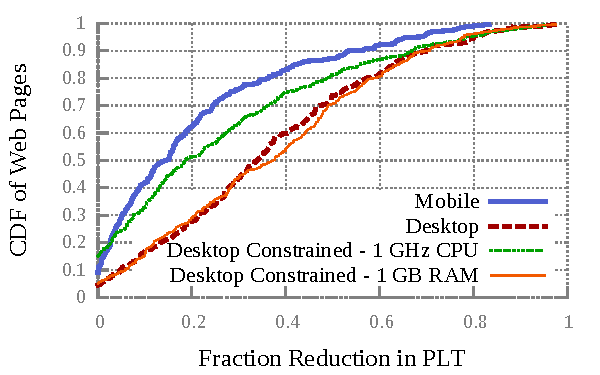
\includegraphics[width=3in]{../graphs/percent_plt_reduction/percent_reduction_linear.pdf}
    \caption[]{\label{fig:percent_reduction_linear}Reduction in page load time due to perfect caching is (significantly) less on mobile devices than desktop. When compared against two resource constrained VMs, CPU appears to be the deciding factor of the effectiveness of CDN caching.}
\end{figure}
We have presented an experimental apparatus for examining the effects of caching on mobile page load time.
Using this apparatus, we demonstrate that mobile page load time is not significantly reduced by caching, contrary to common wisdom.
We go further to show that resource constraints, specifically the CPU, appears to be the main difference between caching's effect on desktop versus mobile.
Content providers may want to reconsider where they focus their optimization efforts, especially as mobile traffic begins to outpace its desktop counterpart.

In future work we plan to measure the critical path on mobile devices, experiment with other web page load time metrics, further levels of caching, and inflating the original network delays to better emulate mobile devices in congested network environments. 

Going forward, mobile devices are becoming increasingly powerful and the bottleneck resources will shift. At what point will web caching have a larger benefit for mobile?  

%\subsection{Future Work}
%There is still space to explore these findings. Using other metrics such as above-the-fold PLT and SpeedIndex may provide deeper insight into the reasoning behind limited mobile PLT reduction. Similarly, examining changes in the critical path with a tool such as WProf would provide valuable insight (WProf does not currently have a mobile tool). 

%It is also worth experimenting with varying levels of caching, namely 22\% and  32\% as in the Google NSDI paper~\cite{flywheel} to see if such incremental changes to mobile PLT are observed. \jamshed{Remove if done.}

%Finally, it is worth adding fixed delays to network responses in order to better emulate mobile and congested networks.
